% Options for packages loaded elsewhere
\PassOptionsToPackage{unicode}{hyperref}
\PassOptionsToPackage{hyphens}{url}
%
\documentclass[
  man]{apa6}
\usepackage{amsmath,amssymb}
\usepackage{iftex}
\ifPDFTeX
  \usepackage[T1]{fontenc}
  \usepackage[utf8]{inputenc}
  \usepackage{textcomp} % provide euro and other symbols
\else % if luatex or xetex
  \usepackage{unicode-math} % this also loads fontspec
  \defaultfontfeatures{Scale=MatchLowercase}
  \defaultfontfeatures[\rmfamily]{Ligatures=TeX,Scale=1}
\fi
\usepackage{lmodern}
\ifPDFTeX\else
  % xetex/luatex font selection
\fi
% Use upquote if available, for straight quotes in verbatim environments
\IfFileExists{upquote.sty}{\usepackage{upquote}}{}
\IfFileExists{microtype.sty}{% use microtype if available
  \usepackage[]{microtype}
  \UseMicrotypeSet[protrusion]{basicmath} % disable protrusion for tt fonts
}{}
\makeatletter
\@ifundefined{KOMAClassName}{% if non-KOMA class
  \IfFileExists{parskip.sty}{%
    \usepackage{parskip}
  }{% else
    \setlength{\parindent}{0pt}
    \setlength{\parskip}{6pt plus 2pt minus 1pt}}
}{% if KOMA class
  \KOMAoptions{parskip=half}}
\makeatother
\usepackage{xcolor}
\usepackage{color}
\usepackage{fancyvrb}
\newcommand{\VerbBar}{|}
\newcommand{\VERB}{\Verb[commandchars=\\\{\}]}
\DefineVerbatimEnvironment{Highlighting}{Verbatim}{commandchars=\\\{\}}
% Add ',fontsize=\small' for more characters per line
\usepackage{framed}
\definecolor{shadecolor}{RGB}{248,248,248}
\newenvironment{Shaded}{\begin{snugshade}}{\end{snugshade}}
\newcommand{\AlertTok}[1]{\textcolor[rgb]{0.94,0.16,0.16}{#1}}
\newcommand{\AnnotationTok}[1]{\textcolor[rgb]{0.56,0.35,0.01}{\textbf{\textit{#1}}}}
\newcommand{\AttributeTok}[1]{\textcolor[rgb]{0.13,0.29,0.53}{#1}}
\newcommand{\BaseNTok}[1]{\textcolor[rgb]{0.00,0.00,0.81}{#1}}
\newcommand{\BuiltInTok}[1]{#1}
\newcommand{\CharTok}[1]{\textcolor[rgb]{0.31,0.60,0.02}{#1}}
\newcommand{\CommentTok}[1]{\textcolor[rgb]{0.56,0.35,0.01}{\textit{#1}}}
\newcommand{\CommentVarTok}[1]{\textcolor[rgb]{0.56,0.35,0.01}{\textbf{\textit{#1}}}}
\newcommand{\ConstantTok}[1]{\textcolor[rgb]{0.56,0.35,0.01}{#1}}
\newcommand{\ControlFlowTok}[1]{\textcolor[rgb]{0.13,0.29,0.53}{\textbf{#1}}}
\newcommand{\DataTypeTok}[1]{\textcolor[rgb]{0.13,0.29,0.53}{#1}}
\newcommand{\DecValTok}[1]{\textcolor[rgb]{0.00,0.00,0.81}{#1}}
\newcommand{\DocumentationTok}[1]{\textcolor[rgb]{0.56,0.35,0.01}{\textbf{\textit{#1}}}}
\newcommand{\ErrorTok}[1]{\textcolor[rgb]{0.64,0.00,0.00}{\textbf{#1}}}
\newcommand{\ExtensionTok}[1]{#1}
\newcommand{\FloatTok}[1]{\textcolor[rgb]{0.00,0.00,0.81}{#1}}
\newcommand{\FunctionTok}[1]{\textcolor[rgb]{0.13,0.29,0.53}{\textbf{#1}}}
\newcommand{\ImportTok}[1]{#1}
\newcommand{\InformationTok}[1]{\textcolor[rgb]{0.56,0.35,0.01}{\textbf{\textit{#1}}}}
\newcommand{\KeywordTok}[1]{\textcolor[rgb]{0.13,0.29,0.53}{\textbf{#1}}}
\newcommand{\NormalTok}[1]{#1}
\newcommand{\OperatorTok}[1]{\textcolor[rgb]{0.81,0.36,0.00}{\textbf{#1}}}
\newcommand{\OtherTok}[1]{\textcolor[rgb]{0.56,0.35,0.01}{#1}}
\newcommand{\PreprocessorTok}[1]{\textcolor[rgb]{0.56,0.35,0.01}{\textit{#1}}}
\newcommand{\RegionMarkerTok}[1]{#1}
\newcommand{\SpecialCharTok}[1]{\textcolor[rgb]{0.81,0.36,0.00}{\textbf{#1}}}
\newcommand{\SpecialStringTok}[1]{\textcolor[rgb]{0.31,0.60,0.02}{#1}}
\newcommand{\StringTok}[1]{\textcolor[rgb]{0.31,0.60,0.02}{#1}}
\newcommand{\VariableTok}[1]{\textcolor[rgb]{0.00,0.00,0.00}{#1}}
\newcommand{\VerbatimStringTok}[1]{\textcolor[rgb]{0.31,0.60,0.02}{#1}}
\newcommand{\WarningTok}[1]{\textcolor[rgb]{0.56,0.35,0.01}{\textbf{\textit{#1}}}}
\usepackage{graphicx}
\makeatletter
\def\maxwidth{\ifdim\Gin@nat@width>\linewidth\linewidth\else\Gin@nat@width\fi}
\def\maxheight{\ifdim\Gin@nat@height>\textheight\textheight\else\Gin@nat@height\fi}
\makeatother
% Scale images if necessary, so that they will not overflow the page
% margins by default, and it is still possible to overwrite the defaults
% using explicit options in \includegraphics[width, height, ...]{}
\setkeys{Gin}{width=\maxwidth,height=\maxheight,keepaspectratio}
% Set default figure placement to htbp
\makeatletter
\def\fps@figure{htbp}
\makeatother
\setlength{\emergencystretch}{3em} % prevent overfull lines
\providecommand{\tightlist}{%
  \setlength{\itemsep}{0pt}\setlength{\parskip}{0pt}}
\setcounter{secnumdepth}{-\maxdimen} % remove section numbering
% Make \paragraph and \subparagraph free-standing
\ifx\paragraph\undefined\else
  \let\oldparagraph\paragraph
  \renewcommand{\paragraph}[1]{\oldparagraph{#1}\mbox{}}
\fi
\ifx\subparagraph\undefined\else
  \let\oldsubparagraph\subparagraph
  \renewcommand{\subparagraph}[1]{\oldsubparagraph{#1}\mbox{}}
\fi
\newlength{\cslhangindent}
\setlength{\cslhangindent}{1.5em}
\newlength{\csllabelwidth}
\setlength{\csllabelwidth}{3em}
\newlength{\cslentryspacingunit} % times entry-spacing
\setlength{\cslentryspacingunit}{\parskip}
\newenvironment{CSLReferences}[2] % #1 hanging-ident, #2 entry spacing
 {% don't indent paragraphs
  \setlength{\parindent}{0pt}
  % turn on hanging indent if param 1 is 1
  \ifodd #1
  \let\oldpar\par
  \def\par{\hangindent=\cslhangindent\oldpar}
  \fi
  % set entry spacing
  \setlength{\parskip}{#2\cslentryspacingunit}
 }%
 {}
\usepackage{calc}
\newcommand{\CSLBlock}[1]{#1\hfill\break}
\newcommand{\CSLLeftMargin}[1]{\parbox[t]{\csllabelwidth}{#1}}
\newcommand{\CSLRightInline}[1]{\parbox[t]{\linewidth - \csllabelwidth}{#1}\break}
\newcommand{\CSLIndent}[1]{\hspace{\cslhangindent}#1}
\ifLuaTeX
\usepackage[bidi=basic]{babel}
\else
\usepackage[bidi=default]{babel}
\fi
\babelprovide[main,import]{english}
% get rid of language-specific shorthands (see #6817):
\let\LanguageShortHands\languageshorthands
\def\languageshorthands#1{}
% Manuscript styling
\usepackage{upgreek}
\captionsetup{font=singlespacing,justification=justified}

% Table formatting
\usepackage{longtable}
\usepackage{lscape}
% \usepackage[counterclockwise]{rotating}   % Landscape page setup for large tables
\usepackage{multirow}		% Table styling
\usepackage{tabularx}		% Control Column width
\usepackage[flushleft]{threeparttable}	% Allows for three part tables with a specified notes section
\usepackage{threeparttablex}            % Lets threeparttable work with longtable

% Create new environments so endfloat can handle them
% \newenvironment{ltable}
%   {\begin{landscape}\centering\begin{threeparttable}}
%   {\end{threeparttable}\end{landscape}}
\newenvironment{lltable}{\begin{landscape}\centering\begin{ThreePartTable}}{\end{ThreePartTable}\end{landscape}}

% Enables adjusting longtable caption width to table width
% Solution found at http://golatex.de/longtable-mit-caption-so-breit-wie-die-tabelle-t15767.html
\makeatletter
\newcommand\LastLTentrywidth{1em}
\newlength\longtablewidth
\setlength{\longtablewidth}{1in}
\newcommand{\getlongtablewidth}{\begingroup \ifcsname LT@\roman{LT@tables}\endcsname \global\longtablewidth=0pt \renewcommand{\LT@entry}[2]{\global\advance\longtablewidth by ##2\relax\gdef\LastLTentrywidth{##2}}\@nameuse{LT@\roman{LT@tables}} \fi \endgroup}

% \setlength{\parindent}{0.5in}
% \setlength{\parskip}{0pt plus 0pt minus 0pt}

% Overwrite redefinition of paragraph and subparagraph by the default LaTeX template
% See https://github.com/crsh/papaja/issues/292
\makeatletter
\renewcommand{\paragraph}{\@startsection{paragraph}{4}{\parindent}%
  {0\baselineskip \@plus 0.2ex \@minus 0.2ex}%
  {-1em}%
  {\normalfont\normalsize\bfseries\itshape\typesectitle}}

\renewcommand{\subparagraph}[1]{\@startsection{subparagraph}{5}{1em}%
  {0\baselineskip \@plus 0.2ex \@minus 0.2ex}%
  {-\z@\relax}%
  {\normalfont\normalsize\itshape\hspace{\parindent}{#1}\textit{\addperi}}{\relax}}
\makeatother

\makeatletter
\usepackage{etoolbox}
\patchcmd{\maketitle}
  {\section{\normalfont\normalsize\abstractname}}
  {\section*{\normalfont\normalsize\abstractname}}
  {}{\typeout{Failed to patch abstract.}}
\patchcmd{\maketitle}
  {\section{\protect\normalfont{\@title}}}
  {\section*{\protect\normalfont{\@title}}}
  {}{\typeout{Failed to patch title.}}
\makeatother

\usepackage{xpatch}
\makeatletter
\xapptocmd\appendix
  {\xapptocmd\section
    {\addcontentsline{toc}{section}{\appendixname\ifoneappendix\else~\theappendix\fi\\: #1}}
    {}{\InnerPatchFailed}%
  }
{}{\PatchFailed}
\keywords{Educational Outcomes, School Quality, Education}
\DeclareDelayedFloatFlavor{ThreePartTable}{table}
\DeclareDelayedFloatFlavor{lltable}{table}
\DeclareDelayedFloatFlavor*{longtable}{table}
\makeatletter
\renewcommand{\efloat@iwrite}[1]{\immediate\expandafter\protected@write\csname efloat@post#1\endcsname{}}
\makeatother
\usepackage{csquotes}
\ifLuaTeX
  \usepackage{selnolig}  % disable illegal ligatures
\fi
\IfFileExists{bookmark.sty}{\usepackage{bookmark}}{\usepackage{hyperref}}
\IfFileExists{xurl.sty}{\usepackage{xurl}}{} % add URL line breaks if available
\urlstyle{same}
\hypersetup{
  pdftitle={An Analysis of the Department of Education Quality Survey and Its Efficacy},
  pdfauthor={Andrew Bowen1, Glen Dale Davis1, Josh Forster1, Shoshana Farber1, \& Charles Ugiagbe1},
  pdflang={en-EN},
  pdfkeywords={Educational Outcomes, School Quality, Education},
  hidelinks,
  pdfcreator={LaTeX via pandoc}}

\title{An Analysis of the Department of Education Quality Survey and Its Efficacy}
\author{Andrew Bowen\textsuperscript{1}, Glen Dale Davis\textsuperscript{1}, Josh Forster\textsuperscript{1}, Shoshana Farber\textsuperscript{1}, \& Charles Ugiagbe\textsuperscript{1}}
\date{}


\shorttitle{DATA621 Final Project}

\affiliation{\vspace{0.5cm}\textsuperscript{1} City University of New York}

\abstract{%
Abstract coming soon!
}



\begin{document}
\maketitle

\hypertarget{introduction}{%
\section{Introduction}\label{introduction}}

The NYC School Survey seeks to collect data to provide an overview of New York City (NYC) Schools. Beginning in 2005, the survey looks to collect demographic and achievement data for New York City Public Schools, and provide a standardized rating of various elements of school quality.

The survey has changed over the years. This change has come from recommendations of public policy analysts in order to more accurately define the quality of schools \emph{New York City Schools (2018)}. The 2020-21 academic year report provides a robust dataset defined at the school level with academic and socioeconomic data provided.

\textbf{Research Question:} This study aims to determine whether the school ratings within the NYC School Quality Survey accurately reflect educational outcomes, or if other variables related to certain schools can be used as a better proxy.

In our case, we are interested in predicting the 4-year college persistence rate for an NYC high school. This measure is defined as the percent of students who graduate from a high school, and eventually go on to graduate from a 4-year colllege. Being able to identify the main indicators of a school's ability to successfully prepare students for college can benefit the NYC Department of Education, and New York City Schools along a couple of dimensions:

\begin{enumerate}
\def\labelenumi{\arabic{enumi}.}
\tightlist
\item
  More directed instruction to enable useful skill transfer in preparatory courses
\item
  Better use of resourcing available to public schools to increase the percentage of college-ready students
\end{enumerate}

For point 2 above, it's well correlated that students who attend 4-year institutions increase their career potential earnings significantly.

\hypertarget{literature-review}{%
\section{Literature Review}\label{literature-review}}

One of the main predictors of academic performance is the socioeconomic background of a student. Students from low-income families are nearly four times more likely to drop out of high school than students from wealthy families \emph{Education Statistics (2008)}.

Attempts to use more sophisticated modeling techniques and different sources datasets come from several prior studies. \emph{Bernacki, Chavez, and Uesbeck (2020)} based their modeling off trying to predict based on student digital behavior, rather than social factors. The model in this study reached an accuracy of 75\%, and was able to flag early interventions. While this modeling technique attempts to predict the same variable (educational achievement, albeit a different metric where we are predicting college attainment), the base dataset used to train the model and input variables are different.

Similarly, \emph{Musso, Cascallar, Bostani, and Crawford (2020)} attempted to train an artificial neural network (ANN) to identify variable relationships to educational performance data. They modeled educational performance of Vietnamese students in grade 5. They included individual characteristics as well as information related to daily routines in their training data. This method uses a more sophisticated model, and resulted in accuracy in prediction of \(95-100%
\) higher than other modeling techniques. However, the training data came in that case from a different country (Vietnam, rather than the United States). Comparing modeling results from this (and other US-centric studies) may not be prudent.

\emph{Yağcı (2022)} predicted final grade exams for Turkish students as well via machine learning models. Their input variables were prior exam grades. These can be a good ``vacuum'' comparison to compare one set of academci performance to another. However, there is a concern that good exam grades (even in one subject) do not correspond to a higher rate of career success later in life \emph{Afarian and Kleiner (2003)}. Additionally, a parent study also found a correlation of up to 0.3 between academic grades and later job performance \emph{Roth, BeVier, Switzer III, and Schippmann (1996)}.

Measuring the input variables that impact educational outcomes is a difficult task. With so many confounding variables, it can be difficult to determine direct causal relationships that have an outsized impact

\hypertarget{data-sourcing}{%
\section{Data Sourcing}\label{data-sourcing}}

The dataset used in this study is published from the \href{https://data.cityofnewyork.us/Education/2020-2021-School-Quality-Reports-High-School/26je-vkp6}{NYC School Quality Report for the Academic Year 2020 - 2021}. It consists of data from 487 New York City public schools, and 391 variables (in the form of columns). This dataset is defined at the school level, indexed by a school's \emph{district borough number} (DBN).

In addition to the school quality ratings provided from survey responses in the data, there is average and raw academic performance data included. In addition to thesea academic indicators, there are socioeconomic variables included as well, such as the percentage of students at a given school in temporary housing services.

\hypertarget{methodology}{%
\section{Methodology}\label{methodology}}

Our primary interest is finding proxy variables within our dataset that can better serve as predictors of 4-year college persistence rates as a given NYC high school than the survey ratings collected by the school quality review. As a result, we'll need to first construct a ``base'' model that predicts a school's college persistence rate.

We can use two variables as a proxy for the school's survey rating in predicting college persistence:

\begin{itemize}
\tightlist
\item
  Percent of Students in Tempoarary Housing (\texttt{temp\_housing\_pct})
\item
  \href{https://data.cccnewyork.org/data/bar/1371/student-economic-need-index\#1371/a/1/1622/127}{Economic Need Index} (\texttt{eni\_hs\_pct\_912}) - this is a measure of the percent of students facing economic hardship at a school \emph{(\textbf{noauthor\_student\_2021?})}. This measures the economic hardship faced by students measured along a few criteria:

  \begin{itemize}
  \tightlist
  \item
    The student is eligible for public assistance from the NYC Human Resources Administration (HRA)
  \item
    The student lived in temporary housing in the past four years
  \item
    The student is in high school, has a home language other than English, and entered the NYC DOE for the first time within the last four years.
  \end{itemize}
\end{itemize}

We create a 20\% holdout set of data to be used later on in order to evaluate the efficacy of our model's predictive capability. The remaining 80\% of the data is to be used for model training and exploratory data analysis (EDA).

For ease of single-node computation, we'll select the variables of interest from our dataset. Notably, these are the survey ratings for each school, as well as our preferred froxy variables. Additionally, we impute both our training and evaluation datasets. Given we are dealing with continuous numeric (and not categorical variables), we use the \emph{Predictive Mean Matching} imputation method native to the R \texttt{mice} package

\begin{verbatim}
## 
##  iter imp variable
##   1   1  survey_pp_CT  survey_pp_RI  survey_pp_ES  survey_pp_SE  survey_pp_SF  survey_pp_TR  college_rate
##   1   2  survey_pp_CT  survey_pp_RI  survey_pp_ES  survey_pp_SE  survey_pp_SF  survey_pp_TR  college_rate
##   1   3  survey_pp_CT  survey_pp_RI  survey_pp_ES  survey_pp_SE  survey_pp_SF  survey_pp_TR  college_rate
##   1   4  survey_pp_CT  survey_pp_RI  survey_pp_ES  survey_pp_SE  survey_pp_SF  survey_pp_TR  college_rate
##   1   5  survey_pp_CT  survey_pp_RI  survey_pp_ES  survey_pp_SE  survey_pp_SF  survey_pp_TR  college_rate
##   2   1  survey_pp_CT  survey_pp_RI  survey_pp_ES  survey_pp_SE  survey_pp_SF  survey_pp_TR  college_rate
##   2   2  survey_pp_CT  survey_pp_RI  survey_pp_ES  survey_pp_SE  survey_pp_SF  survey_pp_TR  college_rate
##   2   3  survey_pp_CT  survey_pp_RI  survey_pp_ES  survey_pp_SE  survey_pp_SF  survey_pp_TR  college_rate
##   2   4  survey_pp_CT  survey_pp_RI  survey_pp_ES  survey_pp_SE  survey_pp_SF  survey_pp_TR  college_rate
##   2   5  survey_pp_CT  survey_pp_RI  survey_pp_ES  survey_pp_SE  survey_pp_SF  survey_pp_TR  college_rate
##   3   1  survey_pp_CT  survey_pp_RI  survey_pp_ES  survey_pp_SE  survey_pp_SF  survey_pp_TR  college_rate
##   3   2  survey_pp_CT  survey_pp_RI  survey_pp_ES  survey_pp_SE  survey_pp_SF  survey_pp_TR  college_rate
##   3   3  survey_pp_CT  survey_pp_RI  survey_pp_ES  survey_pp_SE  survey_pp_SF  survey_pp_TR  college_rate
##   3   4  survey_pp_CT  survey_pp_RI  survey_pp_ES  survey_pp_SE  survey_pp_SF  survey_pp_TR  college_rate
##   3   5  survey_pp_CT  survey_pp_RI  survey_pp_ES  survey_pp_SE  survey_pp_SF  survey_pp_TR  college_rate
##   4   1  survey_pp_CT  survey_pp_RI  survey_pp_ES  survey_pp_SE  survey_pp_SF  survey_pp_TR  college_rate
##   4   2  survey_pp_CT  survey_pp_RI  survey_pp_ES  survey_pp_SE  survey_pp_SF  survey_pp_TR  college_rate
##   4   3  survey_pp_CT  survey_pp_RI  survey_pp_ES  survey_pp_SE  survey_pp_SF  survey_pp_TR  college_rate
##   4   4  survey_pp_CT  survey_pp_RI  survey_pp_ES  survey_pp_SE  survey_pp_SF  survey_pp_TR  college_rate
##   4   5  survey_pp_CT  survey_pp_RI  survey_pp_ES  survey_pp_SE  survey_pp_SF  survey_pp_TR  college_rate
##   5   1  survey_pp_CT  survey_pp_RI  survey_pp_ES  survey_pp_SE  survey_pp_SF  survey_pp_TR  college_rate
##   5   2  survey_pp_CT  survey_pp_RI  survey_pp_ES  survey_pp_SE  survey_pp_SF  survey_pp_TR  college_rate
##   5   3  survey_pp_CT  survey_pp_RI  survey_pp_ES  survey_pp_SE  survey_pp_SF  survey_pp_TR  college_rate
##   5   4  survey_pp_CT  survey_pp_RI  survey_pp_ES  survey_pp_SE  survey_pp_SF  survey_pp_TR  college_rate
##   5   5  survey_pp_CT  survey_pp_RI  survey_pp_ES  survey_pp_SE  survey_pp_SF  survey_pp_TR  college_rate
\end{verbatim}

\begin{verbatim}
## 
##  iter imp variable
##   1   1  survey_pp_CT  survey_pp_RI  survey_pp_SE  college_rate
##   1   2  survey_pp_CT  survey_pp_RI  survey_pp_SE  college_rate
##   1   3  survey_pp_CT  survey_pp_RI  survey_pp_SE  college_rate
##   1   4  survey_pp_CT  survey_pp_RI  survey_pp_SE  college_rate
##   1   5  survey_pp_CT  survey_pp_RI  survey_pp_SE  college_rate
##   2   1  survey_pp_CT  survey_pp_RI  survey_pp_SE  college_rate
##   2   2  survey_pp_CT  survey_pp_RI  survey_pp_SE  college_rate
##   2   3  survey_pp_CT  survey_pp_RI  survey_pp_SE  college_rate
##   2   4  survey_pp_CT  survey_pp_RI  survey_pp_SE  college_rate
##   2   5  survey_pp_CT  survey_pp_RI  survey_pp_SE  college_rate
##   3   1  survey_pp_CT  survey_pp_RI  survey_pp_SE  college_rate
##   3   2  survey_pp_CT  survey_pp_RI  survey_pp_SE  college_rate
##   3   3  survey_pp_CT  survey_pp_RI  survey_pp_SE  college_rate
##   3   4  survey_pp_CT  survey_pp_RI  survey_pp_SE  college_rate
##   3   5  survey_pp_CT  survey_pp_RI  survey_pp_SE  college_rate
##   4   1  survey_pp_CT  survey_pp_RI  survey_pp_SE  college_rate
##   4   2  survey_pp_CT  survey_pp_RI  survey_pp_SE  college_rate
##   4   3  survey_pp_CT  survey_pp_RI  survey_pp_SE  college_rate
##   4   4  survey_pp_CT  survey_pp_RI  survey_pp_SE  college_rate
##   4   5  survey_pp_CT  survey_pp_RI  survey_pp_SE  college_rate
##   5   1  survey_pp_CT  survey_pp_RI  survey_pp_SE  college_rate
##   5   2  survey_pp_CT  survey_pp_RI  survey_pp_SE  college_rate
##   5   3  survey_pp_CT  survey_pp_RI  survey_pp_SE  college_rate
##   5   4  survey_pp_CT  survey_pp_RI  survey_pp_SE  college_rate
##   5   5  survey_pp_CT  survey_pp_RI  survey_pp_SE  college_rate
\end{verbatim}

To check underlying modeling assumptions, we plot distributions and relationships of different variables. First, we plot the distribution of college persistence rates among NYC high schools to check for normality.

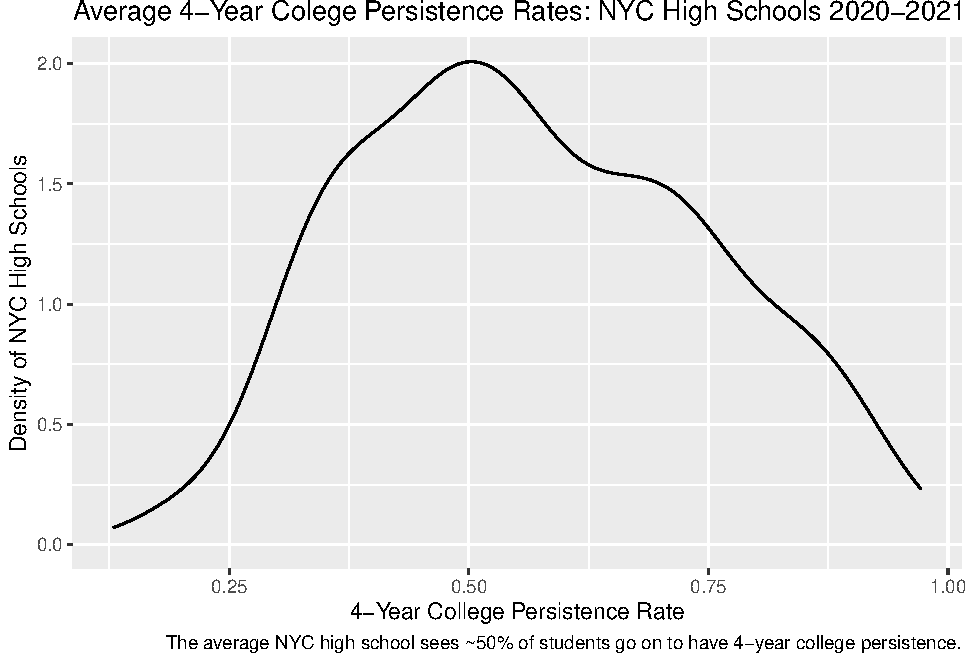
\includegraphics{final-project_files/figure-latex/unnamed-chunk-2-1.pdf}
We see a relatively normal distribution of college persistence rates. In the case of NYC high schools, the peak is at around 50\%. This is inline with national averages released by \emph{US Census Bureau (2023)}

The below plot shows the raw correlation between each variable in our pared down dataset (\emph{Collaborative Teaching}, \emph{Trust}, etc) and the response variable of interest: \emph{4-Year College Persistence Rate}.

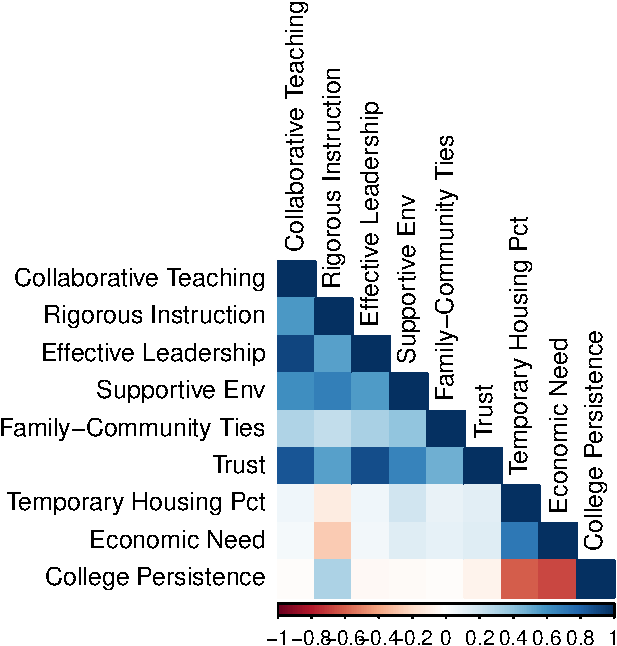
\includegraphics{final-project_files/figure-latex/unnamed-chunk-3-1.pdf}

From our correlation plot above, we can see strong negative relationships between our proxy variables of interest (\emph{Temporary Housing Rate} and \emph{Economic Need Index}) and our target variable: \emph{College Persistence Rate}. This gives signal that constructing models based on these variables could give good insight into the factors that most influence college persistence.

Now we can plot the distributions of our proxy variables of interest. First we can plot the temp housing rate:

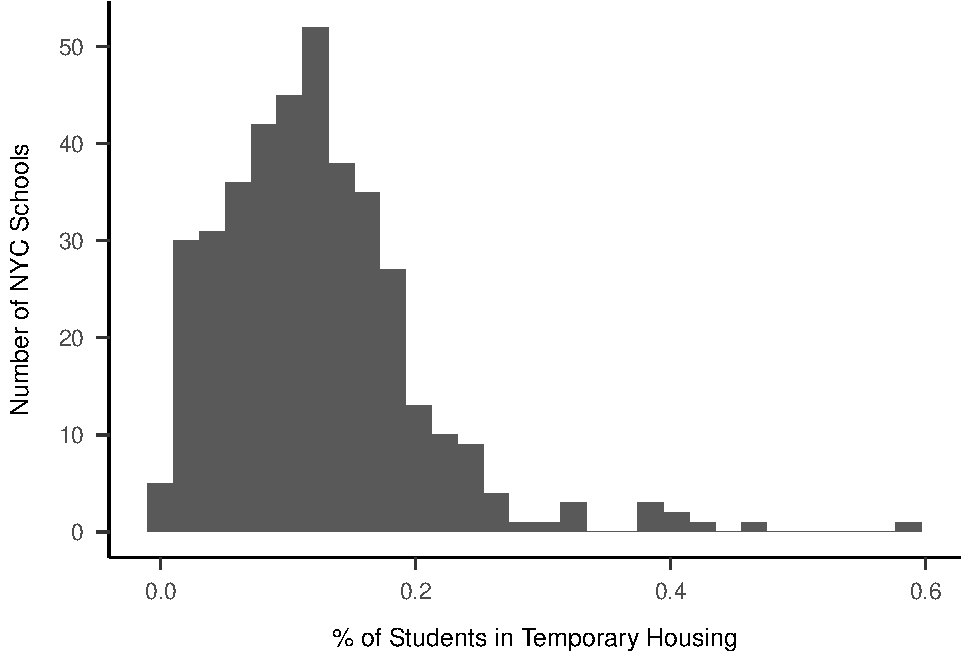
\includegraphics{final-project_files/figure-latex/temp-housing-rates-1.pdf}
We see this distribution of the percentage of students in temporary housing per school to be skewed left. This will be an important piece of information as we model these relationships later. We also show the distribution of schools' economic need indices (also between 0 and 1). This index is closer to 1 the more economic hardship a student at a school faces (temporary housing use or food assistance, for instance).

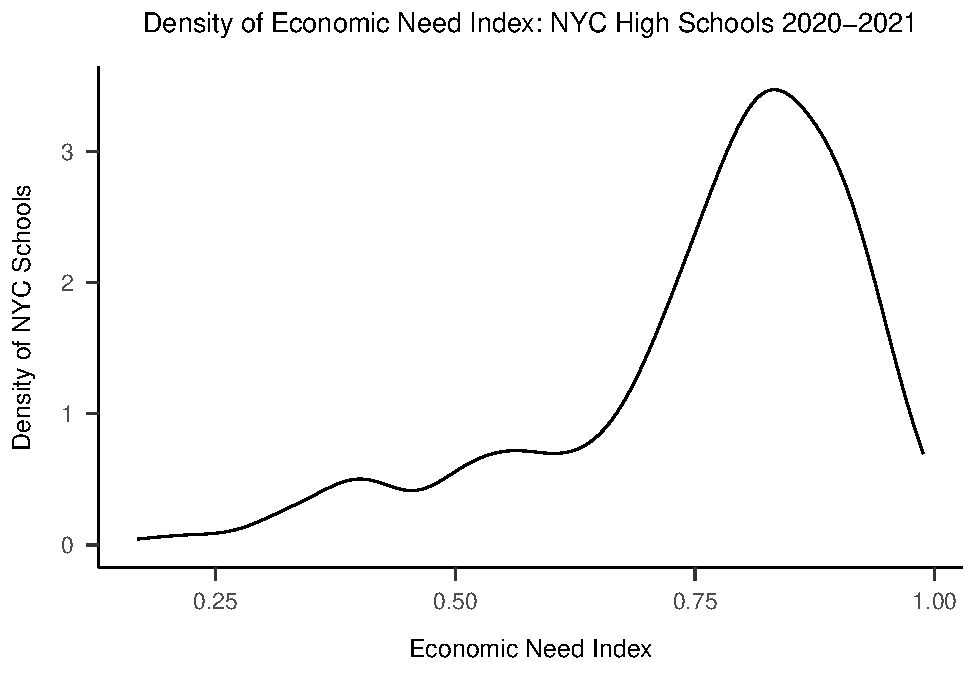
\includegraphics{final-project_files/figure-latex/economic-need-index-1.pdf}
We also see a skewed distribution for our economic need index. This is a candidate for transformation before feeding into our proxy variable model.

First, we should check an assumption of linearity between our predictor and response variables. In this case this a scatter plot of the percentage of students in temporary housing
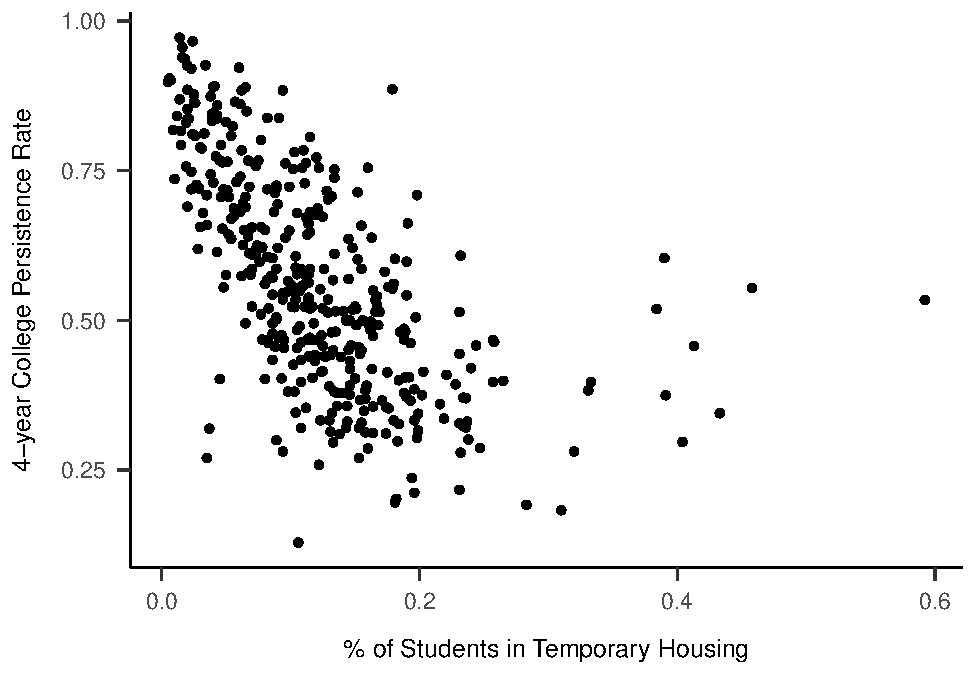
\includegraphics{final-project_files/figure-latex/plot-housing-vs-college-1.pdf}

We see a general linear relationship for schools with lower rates of students in temp housing. However, this linear relationship does \textbf{not} visually hold for schools with higher rates of temp housing use.

Plotting the relationship below between a school's economic need index
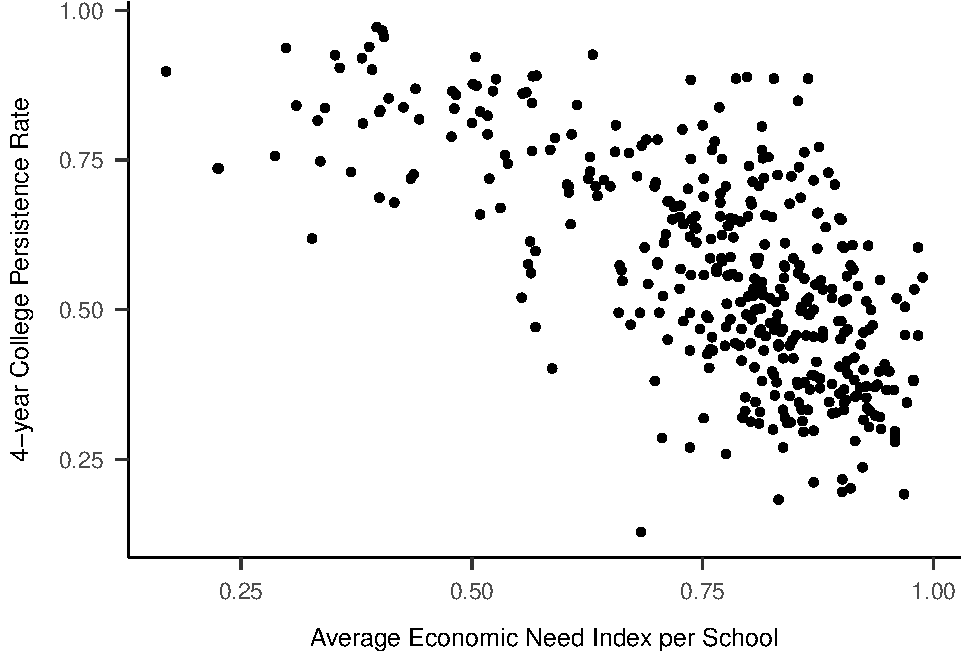
\includegraphics{final-project_files/figure-latex/plot-need-vs-college-1.pdf}
Again, we see a non-linear relationship between our predictor (\emph{Economic Need Index}) and Outcome Variable (\emph{College Persistence Rate})

\hypertarget{modeling}{%
\subsubsection{Modeling}\label{modeling}}

We first create a basic multiple least squares linear model between our two socioeconomic proxy variables: \emph{Temporary Housing PErcentage of a School} and \emph{Average Economic Need Index}.

\begin{verbatim}
## 
## Call:
## lm(formula = proxy_formula, data = train)
## 
## Residuals:
##      Min       1Q   Median       3Q      Max 
## -0.48742 -0.09012  0.00566  0.08315  0.37216 
## 
## Coefficients:
##                  Estimate Std. Error t value Pr(>|t|)    
## (Intercept)       1.04561    0.03621  28.873  < 2e-16 ***
## temp_housing_pct -0.61032    0.12311  -4.958 1.07e-06 ***
## economic_need    -0.53367    0.05893  -9.056  < 2e-16 ***
## ---
## Signif. codes:  0 '***' 0.001 '**' 0.01 '*' 0.05 '.' 0.1 ' ' 1
## 
## Residual standard error: 0.1307 on 387 degrees of freedom
## Multiple R-squared:  0.4786, Adjusted R-squared:  0.4759 
## F-statistic: 177.6 on 2 and 387 DF,  p-value: < 2.2e-16
\end{verbatim}

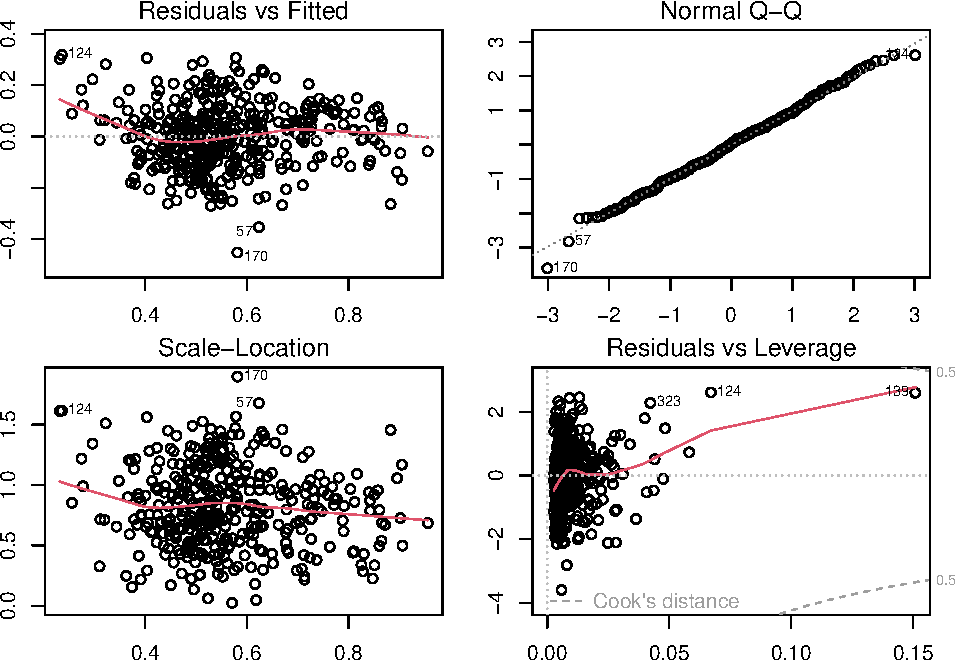
\includegraphics{final-project_files/figure-latex/plot-proxy-model-1.pdf} 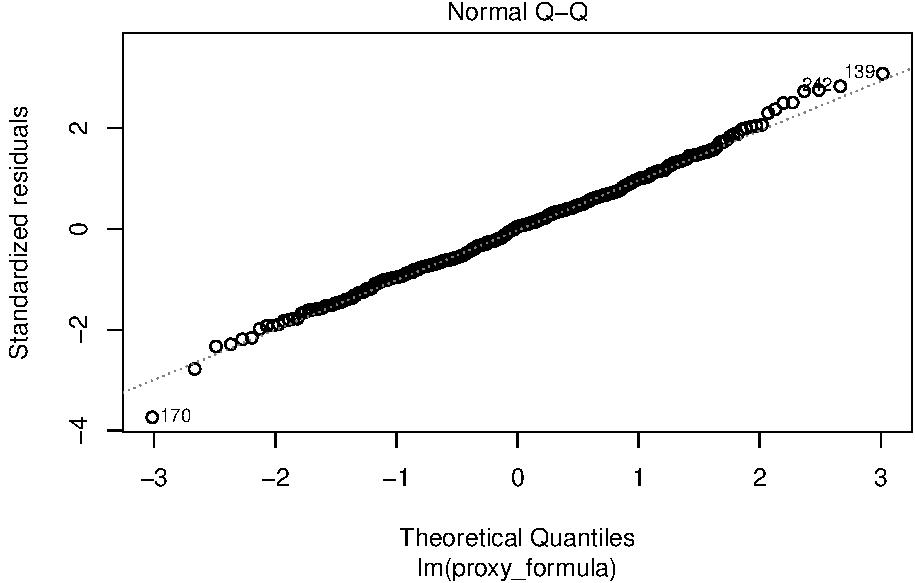
\includegraphics{final-project_files/figure-latex/plot-proxy-model-2.pdf} 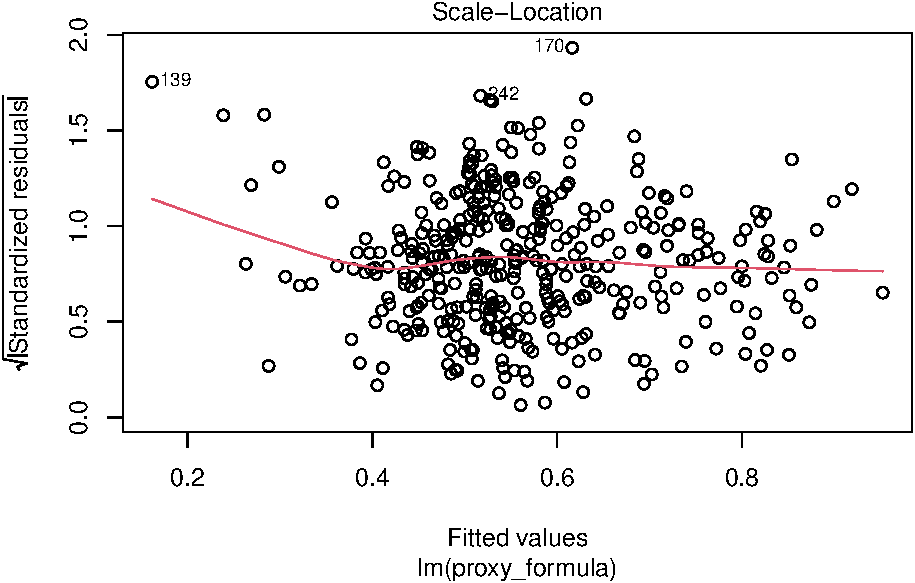
\includegraphics{final-project_files/figure-latex/plot-proxy-model-3.pdf} 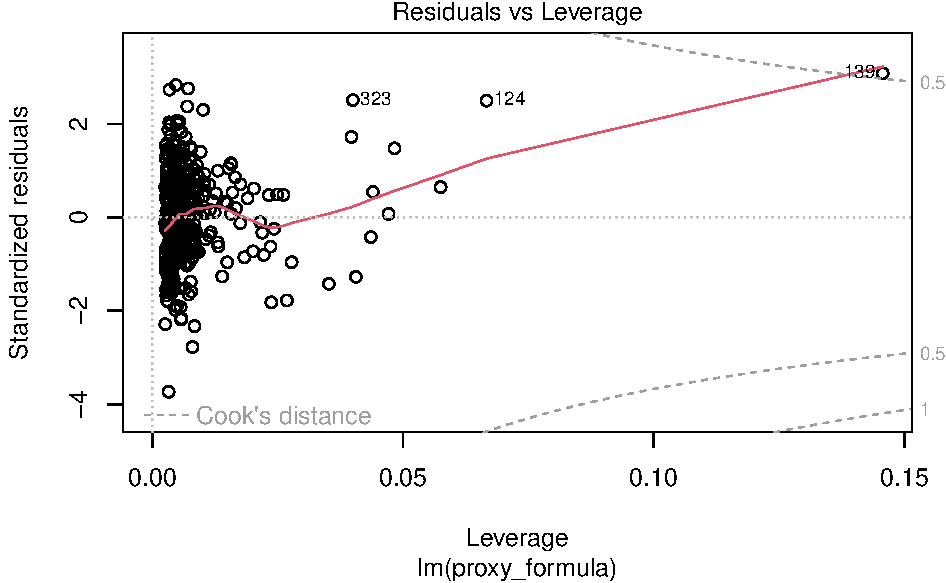
\includegraphics{final-project_files/figure-latex/plot-proxy-model-4.pdf}

Given the

\begin{verbatim}
## 
## Call:
## lm(formula = proxy_formula, data = train, weights = weights)
## 
## Weighted Residuals:
##     Min      1Q  Median      3Q     Max 
## -4.8222 -0.8301  0.0452  0.7834  3.5360 
## 
## Coefficients:
##                  Estimate Std. Error t value Pr(>|t|)    
## (Intercept)       1.02985    0.03260  31.595  < 2e-16 ***
## temp_housing_pct -0.74319    0.13149  -5.652 3.08e-08 ***
## economic_need    -0.49180    0.05594  -8.791  < 2e-16 ***
## ---
## Signif. codes:  0 '***' 0.001 '**' 0.01 '*' 0.05 '.' 0.1 ' ' 1
## 
## Residual standard error: 1.256 on 387 degrees of freedom
## Multiple R-squared:  0.5104, Adjusted R-squared:  0.5078 
## F-statistic: 201.7 on 2 and 387 DF,  p-value: < 2.2e-16
\end{verbatim}

\hypertarget{experimentation-and-results}{%
\section{Experimentation and Results}\label{experimentation-and-results}}

\hypertarget{model-evaluation}{%
\subsubsection{Model Evaluation}\label{model-evaluation}}

\hypertarget{conclusion}{%
\section{Conclusion}\label{conclusion}}

\hypertarget{todo}{%
\subsection{TODO}\label{todo}}

\begin{itemize}
\tightlist
\item
  Merge/Join in ACT/SAT information by DBN
\item
  Model Selection
\end{itemize}

\newpage

\hypertarget{references}{%
\section{References}\label{references}}

\hypertarget{refs}{}
\begin{CSLReferences}{1}{0}
\leavevmode\vadjust pre{\hypertarget{ref-Grades-and-Careers}{}}%
Afarian, R., \& Kleiner, B. (2003). The relationship between grades and career success. \emph{Management Research News}, \emph{26}, 42--51. \url{https://doi.org/10.1108/01409170310783781}

\leavevmode\vadjust pre{\hypertarget{ref-BERNACKI2020103999}{}}%
Bernacki, M. L., Chavez, M. M., \& Uesbeck, P. M. (2020). Predicting achievement and providing support before STEM majors begin to fail. \emph{Computers \& Education}, \emph{158}, 103999. https://doi.org/\url{https://doi.org/10.1016/j.compedu.2020.103999}

\leavevmode\vadjust pre{\hypertarget{ref-NCES-Dropout-Rates}{}}%
Education Statistics, N. C. for. (2008). \emph{Percentage of high school dropouts among persons 16 through 24 years old}. Retrieved from \url{https://nces.ed.gov/programs/digest/d08/tables/dt08_110.asp}

\leavevmode\vadjust pre{\hypertarget{ref-MUSSO202000104}{}}%
Musso, M. F., Cascallar, E. C., Bostani, N., \& Crawford, M. (2020). Identifying reliable predictors of educational outcomes through machine-learning predictive modeling. \emph{Frontiers in Education}, \emph{5}. \url{https://doi.org/10.3389/feduc.2020.00104}

\leavevmode\vadjust pre{\hypertarget{ref-redesign-school-survey}{}}%
New York City Schools, T. R. A. for. (2018). \emph{{R}edesigning the {A}nnual {N}{Y}{C} {S}chool {S}urvey: {L}essons from a {R}esearch-{P}ractice {P}artnership}. \url{https://steinhardt.nyu.edu/sites/default/files/2021-01/Lessons_from_a_Research-Practice_Partnership.pdf}.

\leavevmode\vadjust pre{\hypertarget{ref-roth_meta-analyzing_1996}{}}%
Roth, P. L., BeVier, C. A., Switzer III, F. S., \& Schippmann, J. S. (1996). Meta-analyzing the relationship between grades and job performance. \emph{Journal of Applied Psychology}, \emph{81}(5), 548--556. \url{https://doi.org/10.1037/0021-9010.81.5.548}

\leavevmode\vadjust pre{\hypertarget{ref-CensusBureau_CollegeRates_2023}{}}%
US Census Bureau. (2023). \emph{Census {Cureaur} {Releases} {New} {Educational} {Attainment} {Data}}. Retrieved from \url{https://www.census.gov/newsroom/press-releases/2023/educational-attainment-data.html}

\leavevmode\vadjust pre{\hypertarget{ref-yagci-educational-2022}{}}%
Yağcı, M. (2022). Educational data mining: Prediction of students' academic performance using machine learning algorithms. \emph{Smart Learning Environments}, \emph{9}(1), 11. \url{https://doi.org/10.1186/s40561-022-00192-z}

\end{CSLReferences}

\hypertarget{appendices}{%
\section{Appendices}\label{appendices}}

Below is the code used to generate this report. It's also available on \href{https://github.com/andrewbowen19/businessAnalyticsDataMiningDATA621/main}{GitHub here}

\begin{Shaded}
\begin{Highlighting}[]
\NormalTok{knitr}\SpecialCharTok{::}\NormalTok{opts\_chunk}\SpecialCharTok{$}\FunctionTok{set}\NormalTok{(}\AttributeTok{echo =} \ConstantTok{FALSE}\NormalTok{, }\AttributeTok{warning =} \ConstantTok{FALSE}\NormalTok{, }\AttributeTok{message =} \ConstantTok{FALSE}\NormalTok{)}
\FunctionTok{library}\NormalTok{(tidyverse)}
\FunctionTok{library}\NormalTok{(gridExtra)}
\FunctionTok{library}\NormalTok{(glue)}
\FunctionTok{library}\NormalTok{(mice)}
\FunctionTok{library}\NormalTok{(corrplot)}
\FunctionTok{library}\NormalTok{(}\StringTok{"papaja"}\NormalTok{)}
\FunctionTok{r\_refs}\NormalTok{(}\StringTok{"r{-}references.bib"}\NormalTok{)}
\CommentTok{\# Read in our dataset from GitHub}
\CommentTok{\# https://www.opendatanetwork.com/dataset/data.cityofnewyork.us/bm9v{-}cvch}
\NormalTok{df }\OtherTok{\textless{}{-}} \FunctionTok{read.csv}\NormalTok{(}\StringTok{"https://data.cityofnewyork.us/api/views/26je{-}vkp6/rows.csv?date=20231108"}\NormalTok{)}
\NormalTok{label\_cols }\OtherTok{\textless{}{-}} \FunctionTok{c}\NormalTok{(}\StringTok{"dbn"}\NormalTok{, }\StringTok{"school\_name"}\NormalTok{, }\StringTok{"school\_type"}\NormalTok{)}
\CommentTok{\# Convert needed columns to numeric typing}
\NormalTok{df }\OtherTok{\textless{}{-}} \FunctionTok{cbind}\NormalTok{(df[, label\_cols], }\FunctionTok{as.data.frame}\NormalTok{(}\FunctionTok{lapply}\NormalTok{(df[,}\SpecialCharTok{!}\FunctionTok{names}\NormalTok{(df) }\SpecialCharTok{\%in\%}\NormalTok{ label\_cols], as.numeric)))}

\NormalTok{df}\SpecialCharTok{$}\NormalTok{college\_rate }\OtherTok{\textless{}{-}}\NormalTok{ df}\SpecialCharTok{$}\NormalTok{val\_persist3\_4yr\_all}
\NormalTok{df}\SpecialCharTok{$}\NormalTok{economic\_need }\OtherTok{\textless{}{-}}\NormalTok{ df}\SpecialCharTok{$}\NormalTok{eni\_hs\_pct\_912}
\FunctionTok{set.seed}\NormalTok{(}\DecValTok{42}\NormalTok{)}

\CommentTok{\# Adding a 20\% holdout of our input data for model evaluation later}
\NormalTok{train }\OtherTok{\textless{}{-}} \FunctionTok{subset}\NormalTok{(df[}\FunctionTok{sample}\NormalTok{(}\DecValTok{1}\SpecialCharTok{:}\FunctionTok{nrow}\NormalTok{(df)), ]) }\SpecialCharTok{\%\textgreater{}\%} \FunctionTok{sample\_frac}\NormalTok{(}\FloatTok{0.8}\NormalTok{)}
\NormalTok{test  }\OtherTok{\textless{}{-}}\NormalTok{ dplyr}\SpecialCharTok{::}\FunctionTok{anti\_join}\NormalTok{(df, train, }\AttributeTok{by =} \StringTok{\textquotesingle{}dbn\textquotesingle{}}\NormalTok{)}

\NormalTok{cols }\OtherTok{\textless{}{-}} \FunctionTok{c}\NormalTok{(}\StringTok{"survey\_pp\_CT"}\NormalTok{, }\StringTok{"survey\_pp\_RI"}\NormalTok{,}
          \StringTok{"survey\_pp\_ES"}\NormalTok{, }\StringTok{"survey\_pp\_SE"}\NormalTok{,}
          \StringTok{"survey\_pp\_SF"}\NormalTok{, }\StringTok{"survey\_pp\_TR"}\NormalTok{,}
          \StringTok{"temp\_housing\_pct"}\NormalTok{, }\StringTok{"economic\_need"}\NormalTok{,}
          \StringTok{"college\_rate"}\NormalTok{)}
\NormalTok{train\_data }\OtherTok{\textless{}{-}}\NormalTok{ train[, cols]}
\NormalTok{imp }\OtherTok{\textless{}{-}} \FunctionTok{mice}\NormalTok{(train\_data, }\AttributeTok{method=}\StringTok{"pmm"}\NormalTok{, }\AttributeTok{seed=}\DecValTok{42}\NormalTok{)}
\NormalTok{train }\OtherTok{\textless{}{-}} \FunctionTok{complete}\NormalTok{(imp)}
\NormalTok{test\_data }\OtherTok{\textless{}{-}}\NormalTok{ test[, cols]}
\NormalTok{imp }\OtherTok{\textless{}{-}} \FunctionTok{mice}\NormalTok{(test\_data, }\AttributeTok{method=}\StringTok{"pmm"}\NormalTok{, }\AttributeTok{seed=}\DecValTok{42}\NormalTok{)}
\NormalTok{test }\OtherTok{\textless{}{-}} \FunctionTok{complete}\NormalTok{(imp)}
\CommentTok{\# Plot target variable distribution}
\FunctionTok{ggplot}\NormalTok{(train, }\FunctionTok{aes}\NormalTok{(}\AttributeTok{x=}\NormalTok{college\_rate)) }\SpecialCharTok{+} 
    \FunctionTok{geom\_density}\NormalTok{() }\SpecialCharTok{+} 
    \FunctionTok{labs}\NormalTok{(}\AttributeTok{x=}\StringTok{"4{-}Year College Persistence Rate"}\NormalTok{, }\AttributeTok{y=}\StringTok{"Density of NYC High Schools"}\NormalTok{, }\AttributeTok{title=}\StringTok{"Average 4{-}Year Colege Persistence Rates: NYC High Schools 2020{-}2021"}\NormalTok{, }\AttributeTok{caption=}\StringTok{"The average NYC high school sees \textasciitilde{}50\% of students go on to have 4{-}year college persistence."}\NormalTok{)}

\FunctionTok{theme\_set}\NormalTok{(}\FunctionTok{theme\_apa}\NormalTok{())}

\CommentTok{\# Renaming training dataframe for correlation plot}
\NormalTok{train\_renamed }\OtherTok{\textless{}{-}}\NormalTok{ train }\SpecialCharTok{\%\textgreater{}\%}
  \FunctionTok{rename}\NormalTok{(}\StringTok{"Collaborative Teaching"}\OtherTok{=}\NormalTok{survey\_pp\_CT,}
         \StringTok{"Rigorous Instruction"}\OtherTok{=}\NormalTok{survey\_pp\_RI,}
         \StringTok{"Supportive Env"}\OtherTok{=}\NormalTok{survey\_pp\_SE,}
         \StringTok{"Effective Leadership"}\OtherTok{=}\NormalTok{survey\_pp\_ES,}
         \StringTok{"Family{-}Community Ties"}\OtherTok{=}\NormalTok{survey\_pp\_SF,}
         \StringTok{"Trust"}\OtherTok{=}\NormalTok{survey\_pp\_TR,}
         \StringTok{"Temporary Housing Pct"}\OtherTok{=}\NormalTok{temp\_housing\_pct,}
         \StringTok{"Economic Need"}\OtherTok{=}\NormalTok{economic\_need,}
         \StringTok{"College Persistence"}\OtherTok{=}\NormalTok{college\_rate)}

\CommentTok{\# Create correlation plot between vars of interest}
\NormalTok{corMatrix }\OtherTok{\textless{}{-}} \FunctionTok{cor}\NormalTok{(train\_renamed)}
\FunctionTok{corrplot}\NormalTok{(corMatrix, }\AttributeTok{method=}\StringTok{"color"}\NormalTok{, }\AttributeTok{type=}\StringTok{"lower"}\NormalTok{, }\AttributeTok{tl.col=}\StringTok{"black"}\NormalTok{)}
\CommentTok{\# Plot temp housing rates}
\FunctionTok{ggplot}\NormalTok{(train, }\FunctionTok{aes}\NormalTok{(}\AttributeTok{x=}\NormalTok{temp\_housing\_pct)) }\SpecialCharTok{+}
  \FunctionTok{geom\_histogram}\NormalTok{() }\SpecialCharTok{+}
  \FunctionTok{labs}\NormalTok{(}\AttributeTok{x=}\StringTok{"\% of Students in Temporary Housing"}\NormalTok{, }\AttributeTok{y=}\StringTok{"Number of NYC Schools"}\NormalTok{)}
\CommentTok{\# Plot economic need index}
\FunctionTok{ggplot}\NormalTok{(train, }\FunctionTok{aes}\NormalTok{(}\AttributeTok{x=}\NormalTok{economic\_need)) }\SpecialCharTok{+}
  \FunctionTok{geom\_density}\NormalTok{() }\SpecialCharTok{+}
  \FunctionTok{labs}\NormalTok{(}\AttributeTok{x=}\StringTok{"Economic Need Index"}\NormalTok{, }\AttributeTok{y=}\StringTok{"Density of NYC Schools"}\NormalTok{,}
       \AttributeTok{title=}\StringTok{"Density of Economic Need Index: NYC High Schools 2020{-}2021"}\NormalTok{)}
\CommentTok{\# Plot temp housing percentage vs college persistence rate}
\FunctionTok{ggplot}\NormalTok{(train, }\FunctionTok{aes}\NormalTok{(}\AttributeTok{x=}\NormalTok{temp\_housing\_pct, }\AttributeTok{y=}\NormalTok{college\_rate)) }\SpecialCharTok{+}
  \FunctionTok{geom\_point}\NormalTok{() }\SpecialCharTok{+}
  \FunctionTok{labs}\NormalTok{(}\AttributeTok{x=}\StringTok{"\% of Students in Temporary Housing"}\NormalTok{,}
       \AttributeTok{y=}\StringTok{"4{-}year College Persistence Rate"}\NormalTok{)}
\CommentTok{\# Plot ENI vs college persistence rate}
\FunctionTok{ggplot}\NormalTok{(train, }\FunctionTok{aes}\NormalTok{(}\AttributeTok{x=}\NormalTok{economic\_need, }\AttributeTok{y=}\NormalTok{college\_rate)) }\SpecialCharTok{+}
  \FunctionTok{geom\_point}\NormalTok{() }\SpecialCharTok{+}
  \FunctionTok{labs}\NormalTok{(}\AttributeTok{x=}\StringTok{"Average Economic Need Index per School"}\NormalTok{,}
       \AttributeTok{y=}\StringTok{"4{-}year College Persistence Rate"}\NormalTok{)}
\CommentTok{\# Create OLS linear model based on our proxy variables: no transforms}
\NormalTok{proxy\_formula }\OtherTok{\textless{}{-}}\NormalTok{ college\_rate }\SpecialCharTok{\textasciitilde{}}\NormalTok{ temp\_housing\_pct }\SpecialCharTok{+}\NormalTok{ economic\_need}
\NormalTok{proxy\_model }\OtherTok{\textless{}{-}} \FunctionTok{lm}\NormalTok{(proxy\_formula, train)}
\FunctionTok{summary}\NormalTok{(proxy\_model)}

\FunctionTok{plot}\NormalTok{(proxy\_model)}
\CommentTok{\# Calculating weights for WLS}
\NormalTok{weights }\OtherTok{\textless{}{-}} \DecValTok{1} \SpecialCharTok{/} \FunctionTok{lm}\NormalTok{(}\FunctionTok{abs}\NormalTok{(proxy\_model}\SpecialCharTok{$}\NormalTok{residuals) }\SpecialCharTok{\textasciitilde{}}\NormalTok{ proxy\_model}\SpecialCharTok{$}\NormalTok{fitted.values)}\SpecialCharTok{$}\NormalTok{fitted.values}\SpecialCharTok{\^{}}\DecValTok{2}

\CommentTok{\#perform weighted least squares regression}
\NormalTok{wls\_model }\OtherTok{\textless{}{-}} \FunctionTok{lm}\NormalTok{(proxy\_formula, }\AttributeTok{data =}\NormalTok{ train, }\AttributeTok{weights=}\NormalTok{weights)}

\FunctionTok{summary}\NormalTok{(wls\_model)}
\end{Highlighting}
\end{Shaded}


\end{document}
